\section{Evaluation}
\label{sec:eval}

We evaluate the performance of ChimeraTL in terms of the accuracy of the performance prediction model it builds.
We compare ChimeraTL with the following four methods: \textit{ModelShift}, \textit{DataReuseTL}, \textit{L2S}, and \textit{L2S+DataReuseTL} (a combined approach of DataReuseTL and L2S\cite{l2s}). 

Although original papers of ModelShift and DataReuseTL do not conduct parameter selection, we perform parameter selection using stepwise regression\cite{stepwise} for these methods to achieve the best performance.
In addition, we use the same Gaussian Process regression model as the performance prediction model for all the methods to ensure a fair comparison of transfer learning approaches.

\subsection{Experimental Setup}
\label{sec:eval:setup}
For all the experiments, we use LineairDB\cite{lineairdb} to generate performance data.
LineairDB~\cite{lineairdb} is an open-source transactional key-value storage engine based on Silo~\cite{silo}.
% LineairDB incorporates NWR~\cite{nakazono} in its implementation of optimistic concurrency control. 
% In addition, it provides efficient logging by epoch-based group commit. 
% Both of these factors support LineairDB's high performance and scalability for various workloads in many-core environments.
The parameter space of LineairDB considered in this paper is shown in Table~\ref{tab:lineairdb}.
\begin{table}[t]
    \caption{Parameter space of LineairDB}
    \label{tab:lineairdb}
    \centering
    \begin{tabular}{|c|c|c|}
        \hline
        \textbf{Parameter} & \textbf{Range} & \textbf{Default value} \\
        \hline
        \texttt{clients} & 1-24 & 1 \\
        \hline
        \texttt{checkpoint\_interval} & 1-30 & 30 \\
        \hline
        \texttt{epoch\_duration} & 1-40 & 40 \\
        \hline
        \texttt{prefetch\_locality} & 0-3 & 3 \\
        \hline
        \texttt{rehash\_threshold} & 0.1-0.99 & 0.8 \\
        \hline
    \end{tabular}
\end{table}

Table \ref{tab:env} shows the source and target environments used in the experiments.
For the source environment, we set up a docker container on a MacBook Pro with Apple M3 Max processor (16 cores) and 48 GB memory.
Conversely, we use a server with Intel(R) Xeon(R) Gold 6130 CPU (2.10GHz, 64 cores) and 1.6 TB memory to host a docker container for the target environment.
Docker containers are used to restrict the amount of resources available to each environment.
We use two completely different host machines to simulate the case where developers test their software on a local machine and deploy it on a server.

\begin{table}[tb]
    \caption{Source and target environments}
    \label{tab:env}
    \centering
    \begin{tabular}{|c|c|c|}
        \hline
        \textbf{Environment} & \textbf{Source} & \textbf{Target} \\
        \hline
        \textbf{\#Cores} & 8 & 24 \\
        \hline
        \textbf{RAM size} & 12 GB & 32 GB \\
        \hline
        \textbf{Host Machine CPU} & Apple M3 Max &  Intel(R) Xeon(R) Gold 6130 \\
        & (16 cores) & (64 cores) \\
        \hline
        \textbf{Host Machine RAM size} & 48GB & 1.6TB \\
        \hline
    \end{tabular}
\end{table}

We measure the performance of LineairDB by running the Yahoo! Cloud Serving Benchmark (YCSB)\cite{ycsb} with the workload A.
In all the experiments, we assume that the workload is the same between the source and target environments.
This assumption is realistic because application developers test their software for expected workloads before deploying it to the target environment.
For the performance metric, we use the throughput of the database, which is the number of transactions processed per second.

% Since the goal of this paper is to propose a transfer learning method that can build an accurate performance prediction model with fewer samples from the target environment, we evaluate each transfer learning method in terms of the number of samples required to build a model with a certain accuracy.
% As the accuracy metric, we use mean absolute percentage error (MAPE), which is defined as follows:
% \begin{equation}
%     \label{eq:mape}
%     \text{MAPE} = \frac{1}{n}\sum_{i=1}^{n}\left|\frac{y_i - \hat{y}_i}{y_i}\right|
% \end{equation}
% where $y_i$ is the actual performance of the $i$-th sample, $\hat{y}_i$ is the predicted performance of the $i$-th sample, and $n$ is the number of samples.
% MAPE is a common scale-independent metric for evaluating the accuracy of performance prediction models\cite{Valov, l2s, mape}.
% We run each experiment 5 times and calculate the average MAPE.

\subsection{Comparison with Existing Methods}
\label{sec:eval:exst}
% \begin{figure*}[th]
%     \centering 
%     \begin{minipage}{.325\textwidth}
%         \centering
%         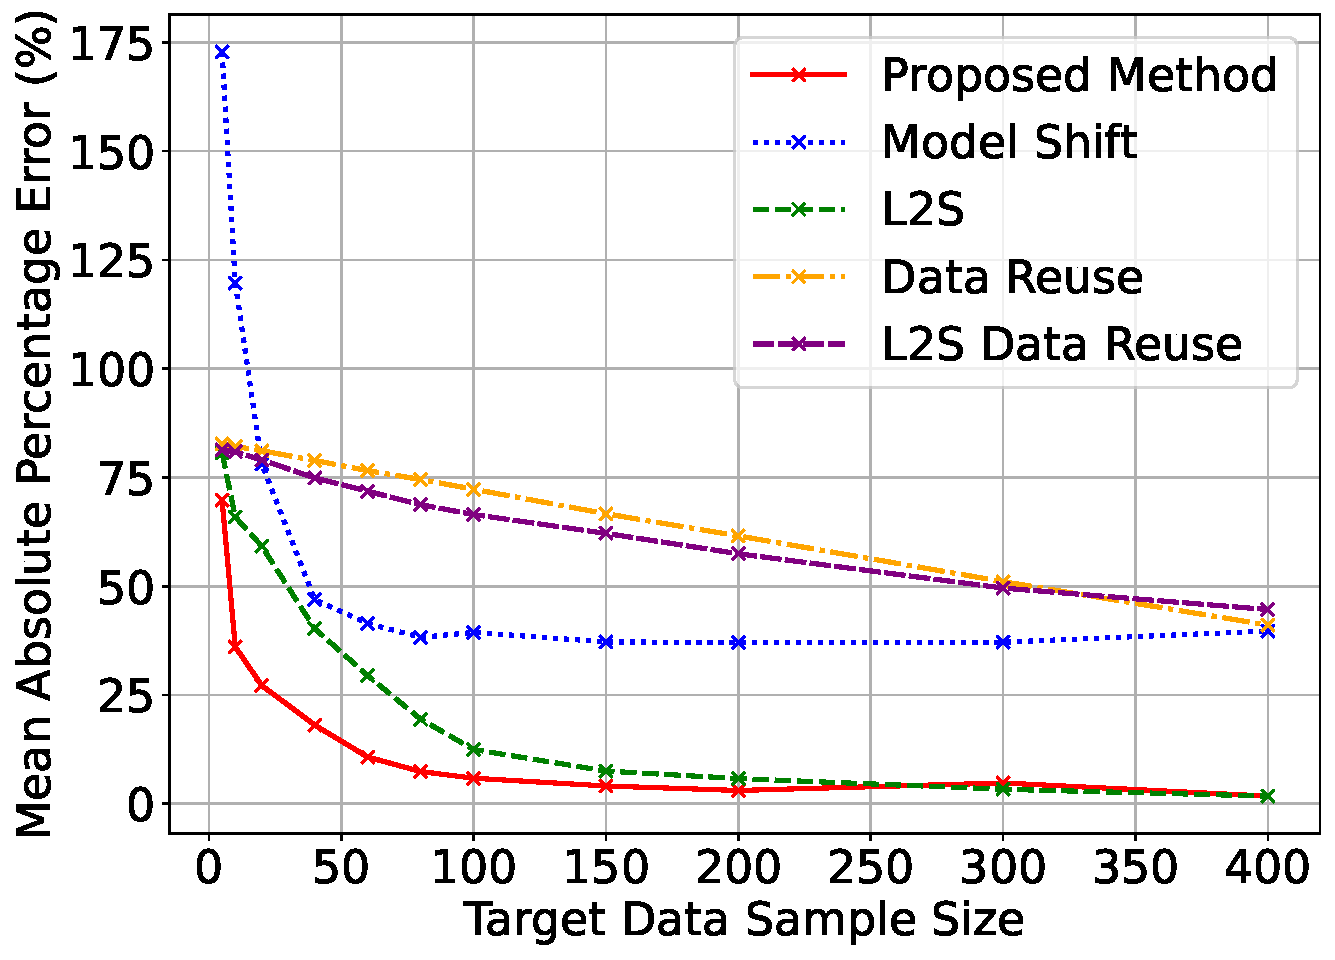
\includegraphics[width=.9\linewidth]{src/fig/tl.pdf}
%         \caption{\textbf{Performance prediction accuracy of transfer learning methods}}
%         \label{fig:results}
%     \end{minipage}
%     \hfill
%     \begin{minipage}{.325\textwidth}
%         \centering
%         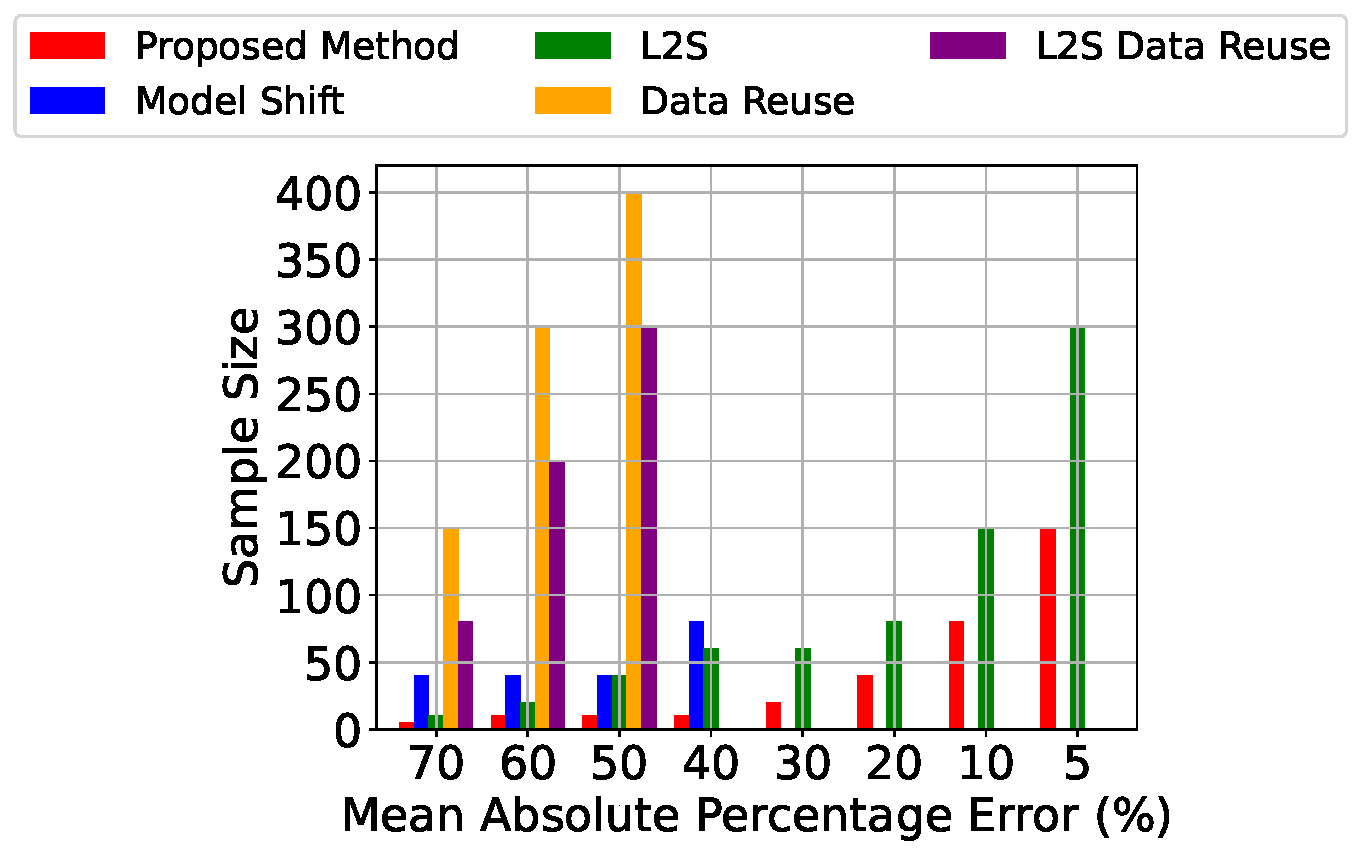
\includegraphics[width=1\linewidth]{src/fig/tl_bar.pdf}
%         \caption{\textbf{Minimum samples required for improved prediction accuracy} -- ModelShift, DataReuseTL, and L2S+DataReuseTL cannot reduce the error below 40\% even with all the samples from the target environment.}
%         \label{fig:bar}
%     \end{minipage}
%     \hfill
%     \begin{minipage}{.325\textwidth}
%         \centering
%         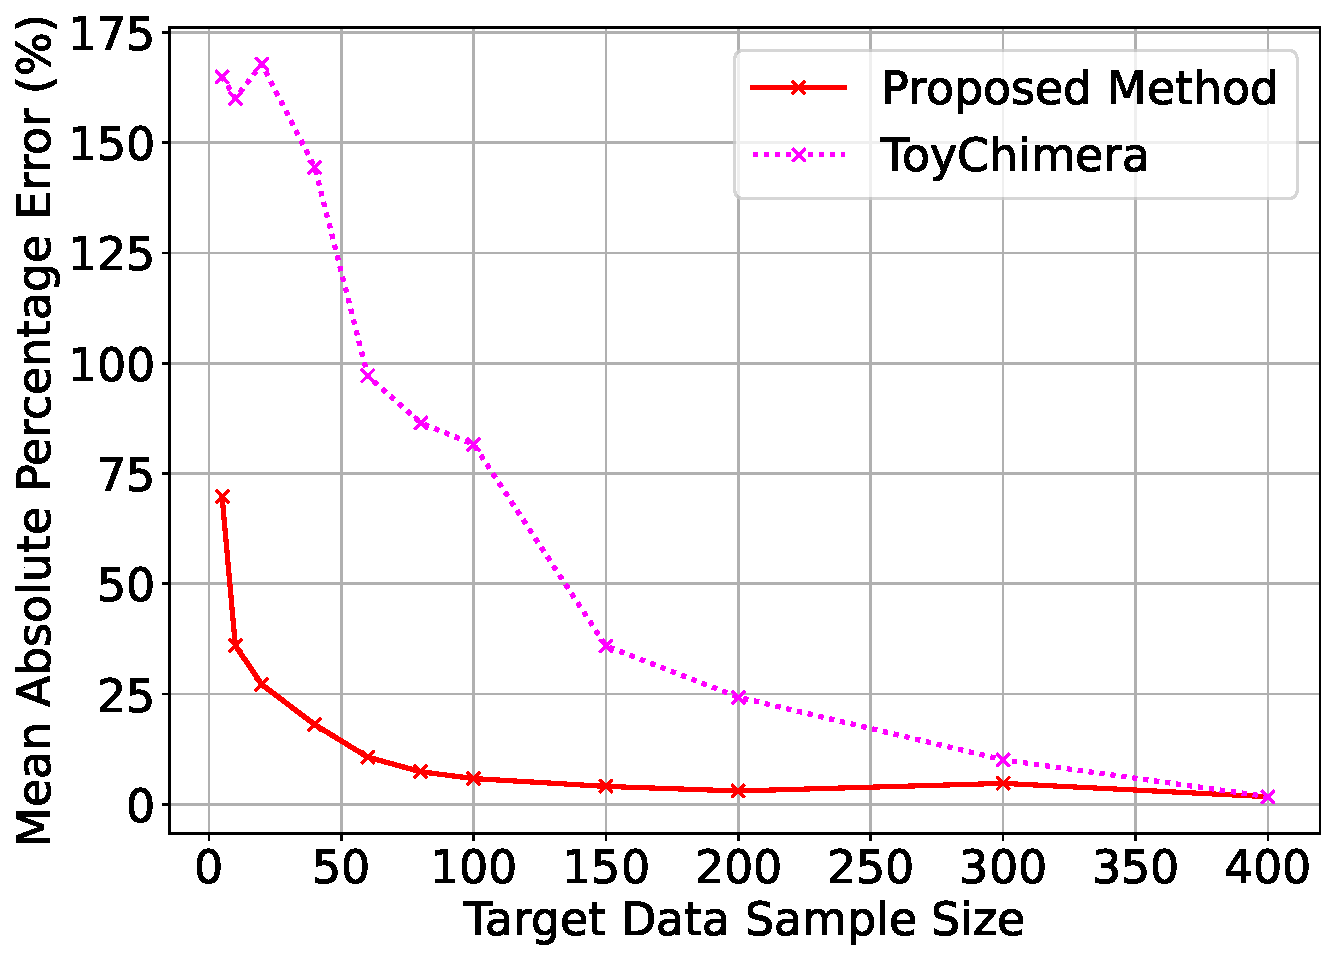
\includegraphics[width=.9\linewidth]{src/fig/toy.pdf}
%         \caption{\textbf{Performance prediction accuracy of ChimeraTL and ToyChimera}}
%         \label{fig:toy}
%     \end{minipage}
% \end{figure*}
% \begin{figure*}[th]
%     \centering
%     \begin{minipage}{.45\textwidth}
%         \centering
%         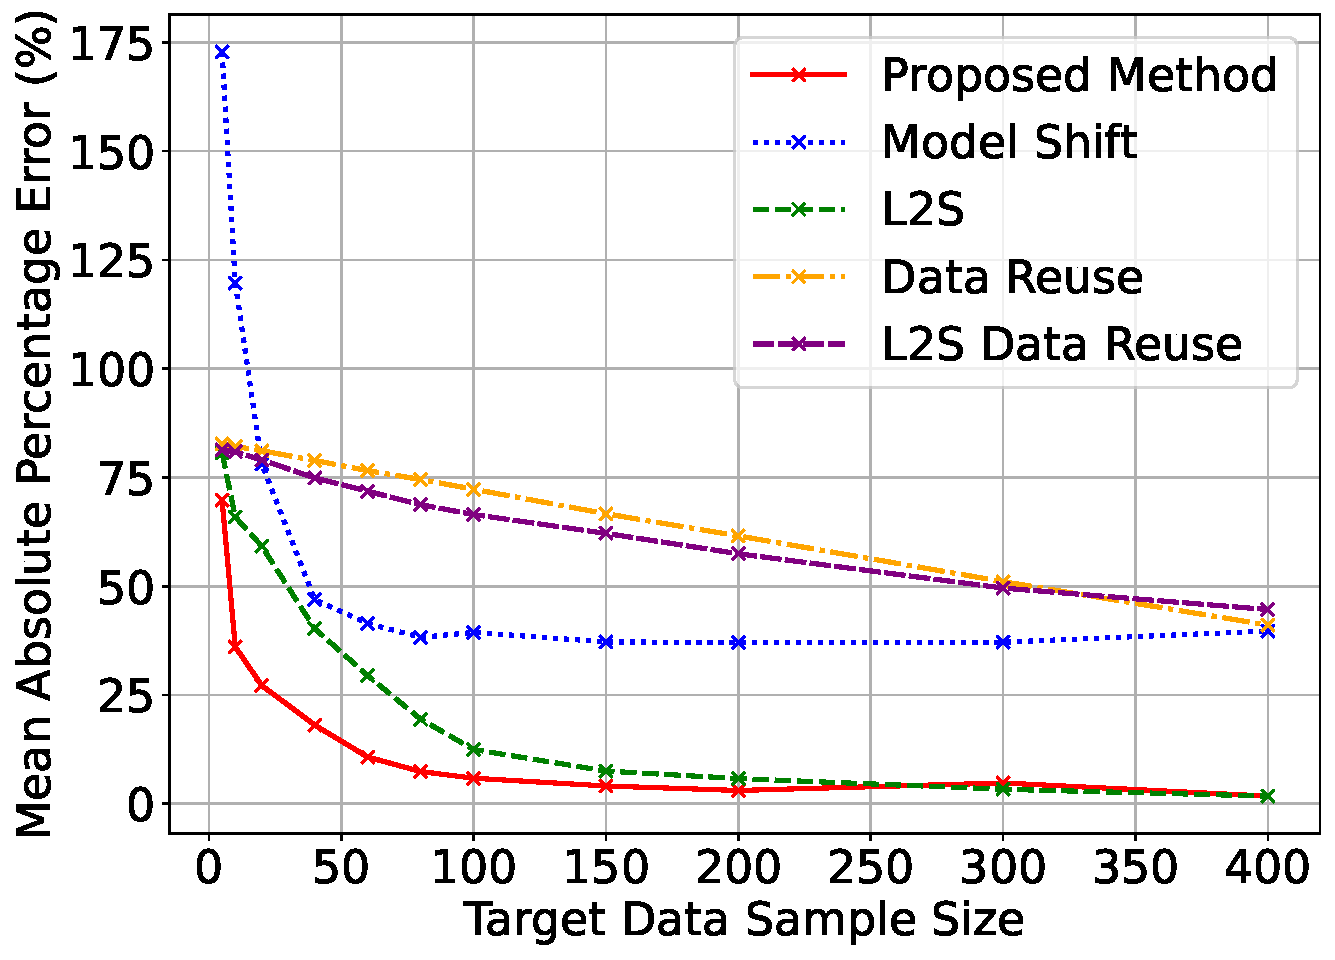
\includegraphics[width=.7\linewidth]{src/fig/tl.pdf}
%         \caption{\textbf{Performance prediction accuracy of transfer learning methods}}
%         \label{fig:results}
%     \end{minipage}%
%     \hfill
%     \begin{minipage}{.45\textwidth}
%         \centering
%         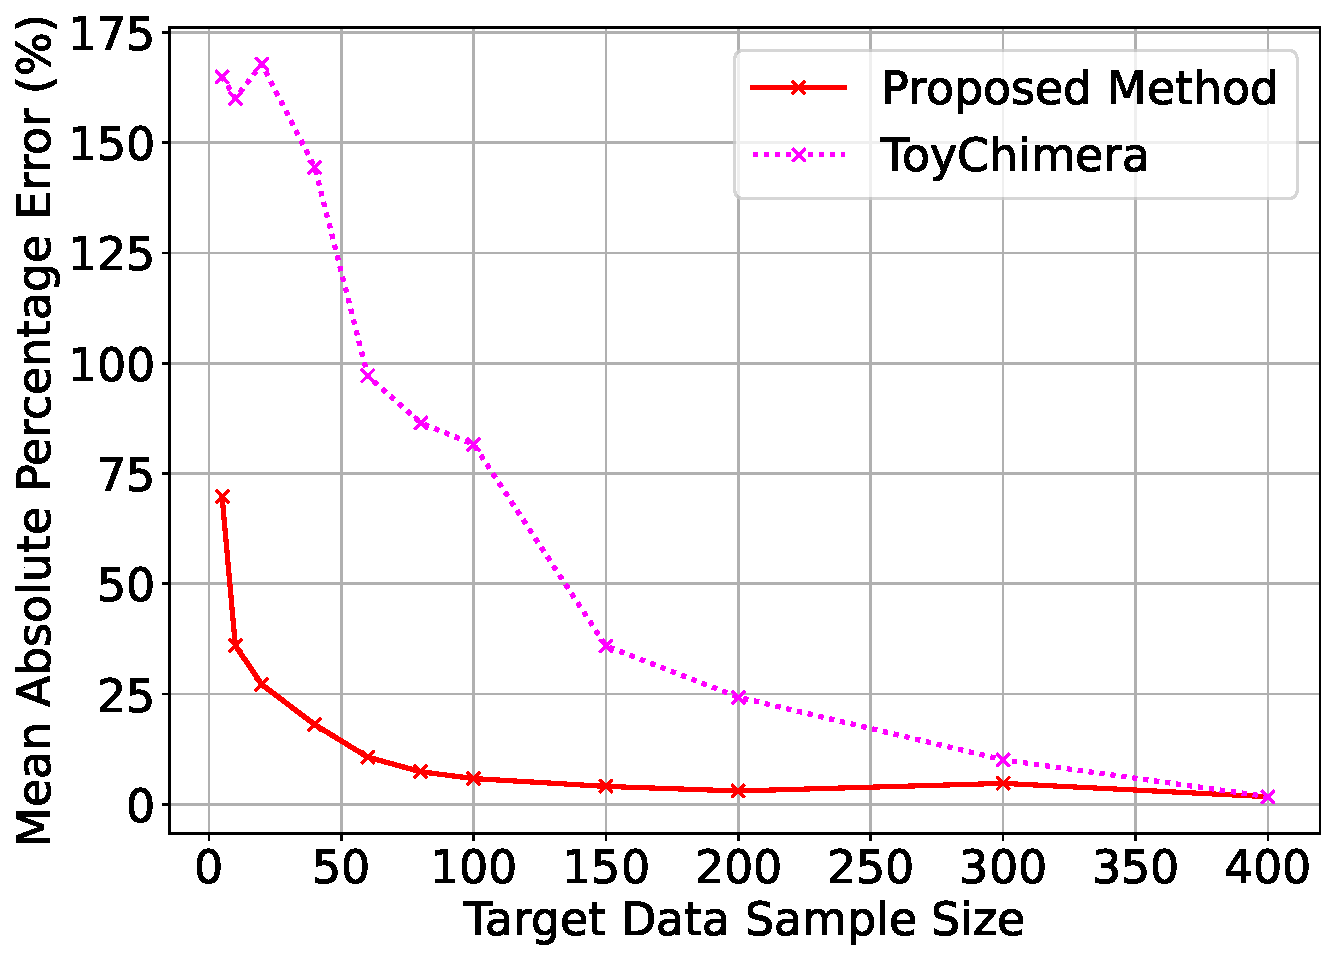
\includegraphics[width=.7\linewidth]{src/fig/toy.pdf}
%         \caption{\textbf{Performance prediction accuracy of ChimeraTL and ToyChimera}}
%         \label{fig:toy}
%     \end{minipage}
% \end{figure*}
\begin{figure*}[th]
    \centering
    \begin{minipage}{.45\textwidth}
        \centering
        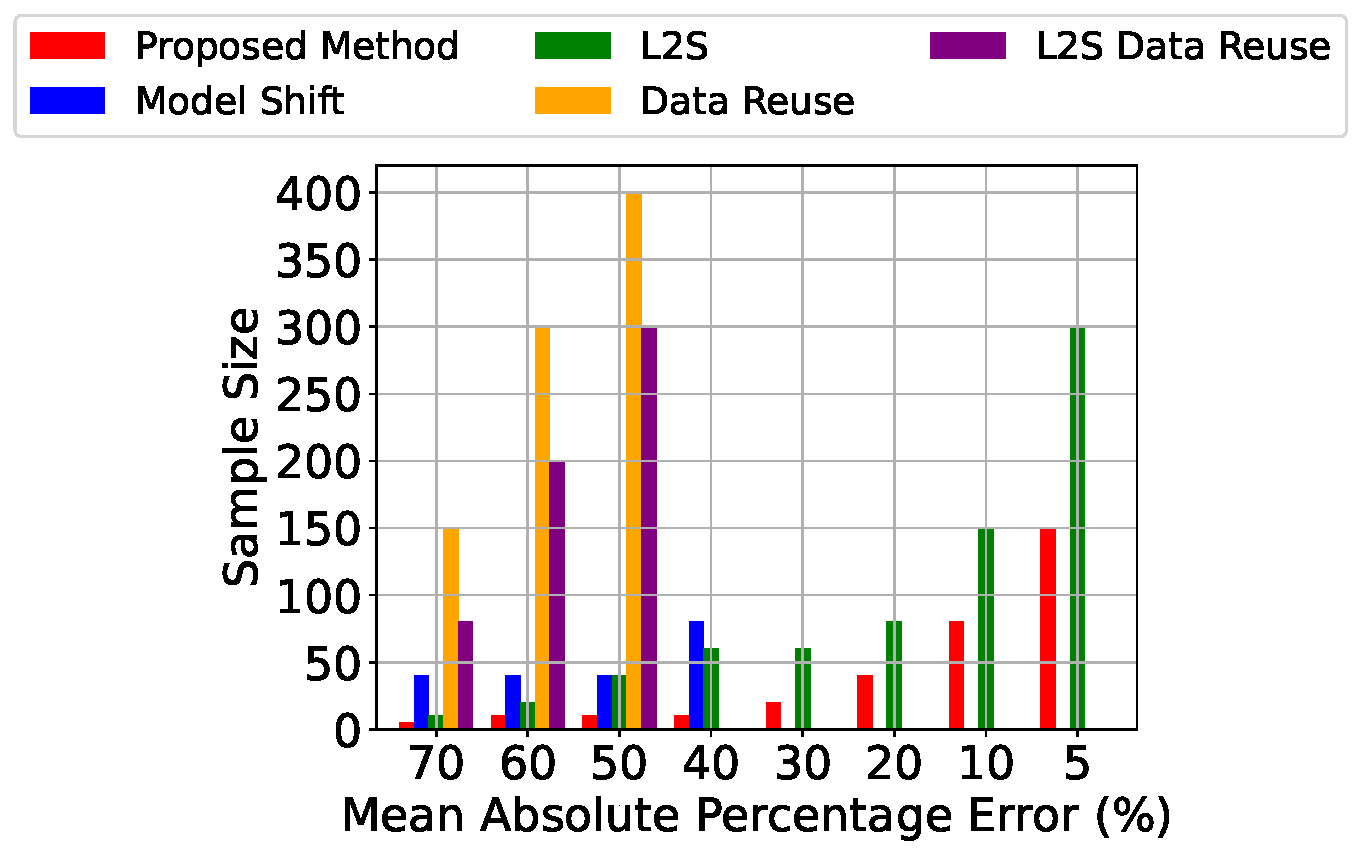
\includegraphics[width=1\linewidth]{src/fig/tl_bar.pdf}
        \caption{\textbf{Performance prediction accuracy of transfer learning methods} -- ModelShift, DataReuseTL, and L2S+DataReuseTL cannot reduce the error below 40\% even with all the samples from the target environment.}
        \label{fig:results}
    \end{minipage}%
    \hfill
    \begin{minipage}{.45\textwidth}
        \centering
        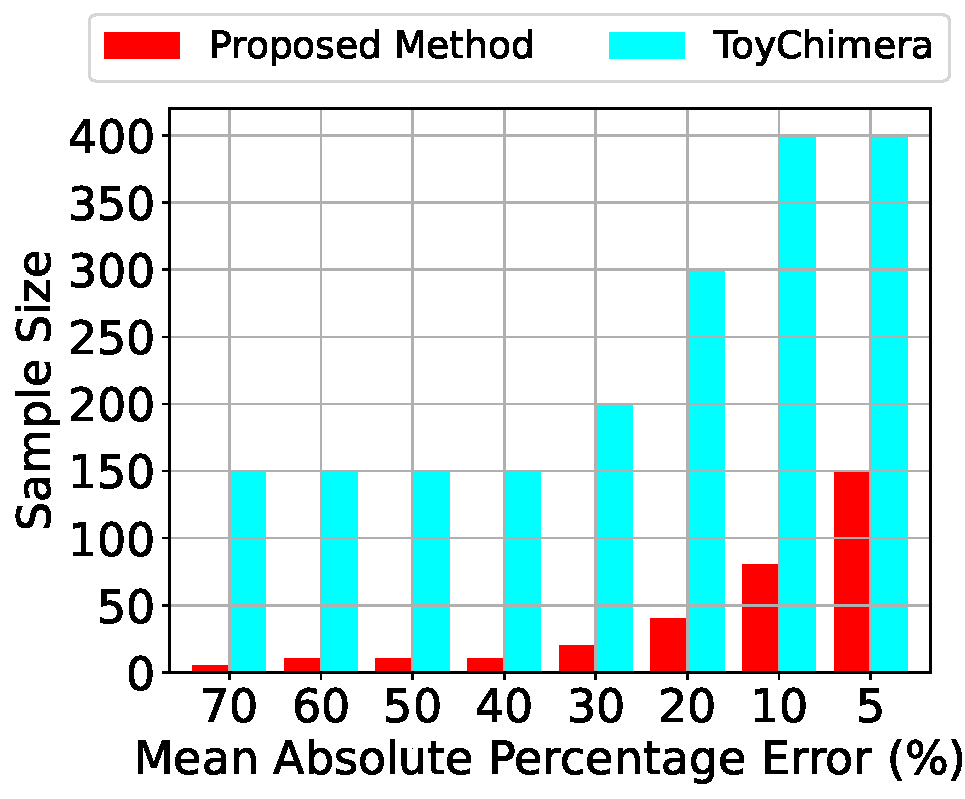
\includegraphics[width=.7\linewidth]{src/fig/toy_bar.pdf}
        \caption{\textbf{Performance prediction accuracy of ChimeraTL and ToyChimera}}
        \label{fig:toy}
    \end{minipage}
\end{figure*}

Fig.~\ref{fig:results} shows the performance prediction accuracy of the transfer learning methods.
The x-axis represents the number of samples from the target environment and the y-axis represents the mean absolute percentage error (MAPE)\cite{Valov, l2s, mape} of the performance prediction model.

While the existing methods do not show a large difference with 10 samples, ChimeraTL already separates itself from the other methods, reducing the prediction error to below 40\%.
This result demonstrates the effectiveness of ChimeraTL's linear transformation learning that aims to linearly transform and reuse the source data for the target model construction.
ChimeraTL further reduces the prediction error to under 10\% with 80 samples, while other methods require at least 150 samples to achieve the same accuracy.
ChimeraTL's steady improvement in prediction accuracy with increased number of samples justifies its strategy to prioritize sampling for non-linear parameters once enough samples are collected for the linear transformation learning.
With ChimeraTL achieving the best prediction accuracy for almost all the number of samples, it is clear that ChimeraTL can build an accurate performance prediction model with fewer samples from the target environment. 

Contrary to the findings of the previous work that ModelShift needs less than 10 samples to learn the linear transformation\cite{Valov}, ModelShift requires 80 samples to achieve its best prediction accuracy of just around 40\% in our experiments.
This is because there are non-linear parameters in LineairDB that interfere with the learning of the linear transformation.
DataReuseTL and L2S+DataReuseTL display steady improvement in prediction accuracy, but their prediction accuracy never reaches below 40\% even with all available samples from the target environment because there is a huge difference between the DBMS performance in the source and target environments.
Even though ChimeraTL linearly transforms the source data and reuses it for the target model construction, the effect of negative transfer is minimized because ChimeraTL excludes the source data of non-linear parameters in the process.

Contrasting with the methods that suffer from the negative transfer, L2S shows a steady improvement in prediction accuracy as the number of samples increases.
Still, L2S generally requires twice as many samples as ChimeraTL to achieve the same prediction accuracy.
Since L2S does not use the source environment data at all to train the model, it requires more samples from the target environment to build a model with the same accuracy as ChimeraTL.

\subsection{Importance of Parameter Separation}
To understand the effect of parameter separation, we compare ChimeraTL with ToyChimera, a variant of ChimeraTL that does not separate parameters.
Essentially, ToyChimera is the same as ChimeraTL except (1) it does not exclude the data of non-linear parameters from the linear transformation learning and the source data reuse, and (2) it samples data randomly instead of giving priority to certain parameters at different stages of the sampling process.
Fig.~\ref{fig:toy} shows the performance prediction accuracy of ChimeraTL and ToyChimera, in addition to the baseline method.
% \begin{figure}[t]
%     \centering
%     \centerline{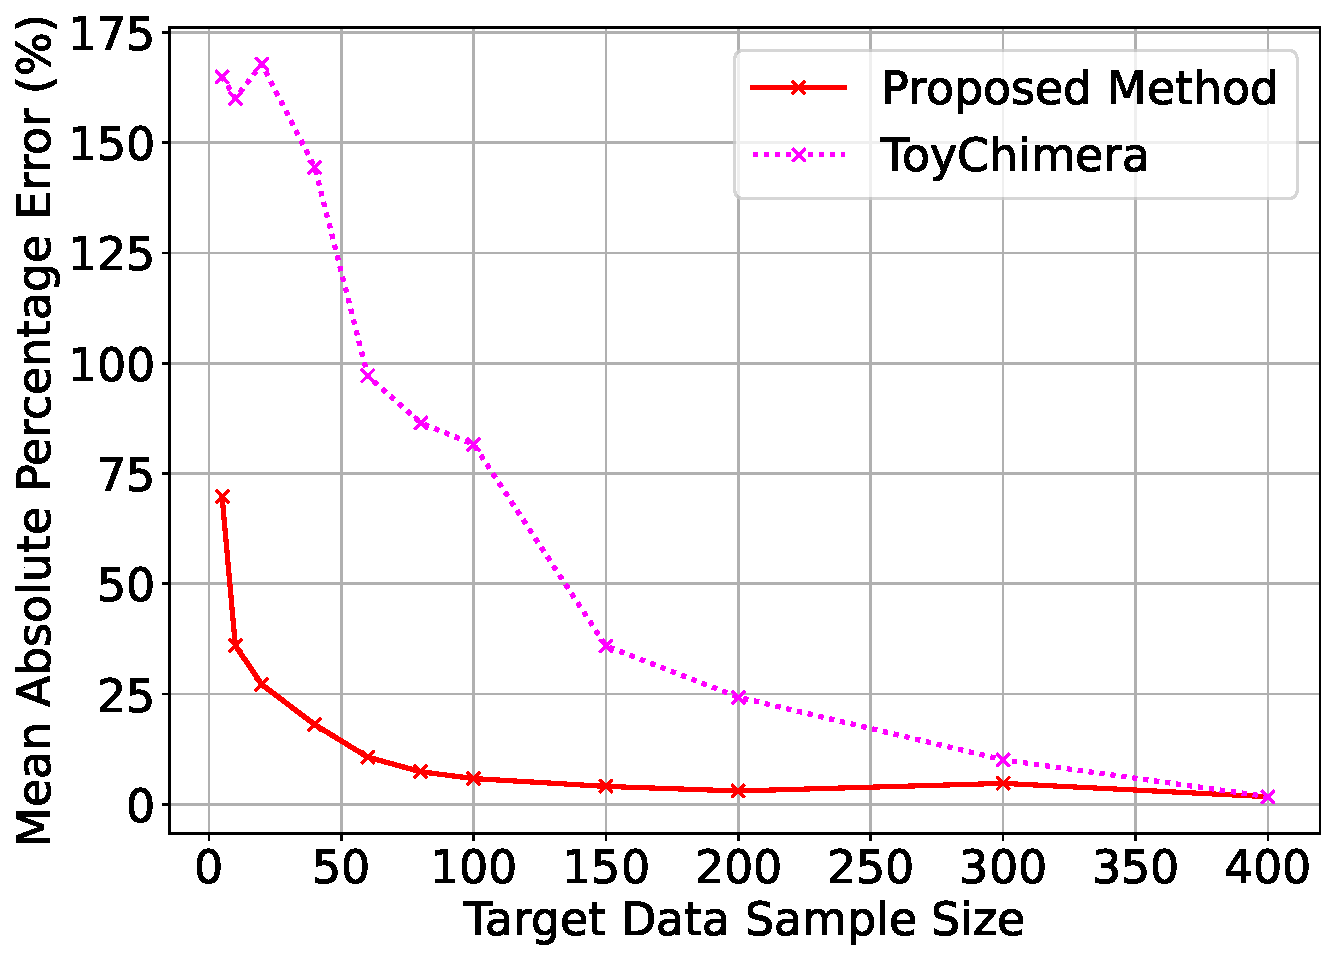
\includegraphics[width=0.475\textwidth]{src/fig/toy.pdf}}
%     \caption{\textbf{Performance prediction accuracy of ChimeraTL and ToyChimera}}
%     \label{fig:toy}
% \end{figure}

As shown in Fig.~\ref{fig:toy}, The prediction accuracy of ToyChimera significantly falls short when compared to that of ChimeraTL.
ToyChimera can only reduce the error to around 35\% with 150 samples, when ChimeraTL can reduce the error to below 5\% with the same number of samples.

As explained in Section~\ref{sec:eval:exst} and shown in Fig.~\ref{fig:results}, involving non-linear parameters in the linear transformation learning and reusing all the source data causes the negative transfer which significantly degrades the prediction accuracy.
ChimeraTL filters out the data of non-linear parameters for these processes so that it can reuse the source data without suffering from the negative transfer.
Consequently, ChimeraTL can build a more accurate performance prediction model with fewer samples from the target environment.